\section{Arquitectura}
En esta sección mostraremos los diagramas (\textbf{vista C\&C}) desarrollados para la arquitectura del sistema. Por razones de claridad y espacio, se omitió en el diagrama el detalle de los puertos y roles en los componentes y conectores.

Consideramos nuestra arquitectura con un estilo predominantemente Cliente-Servidor, donde el Servidor es nuestro sistema, distribuido en distintas máquinas (\textit{nodos}) a través del mundo, mientras que el Cliente es el navegador web que se encuentra en el dispositivo que utiliza el usuario.

\subsection{Paneo General}
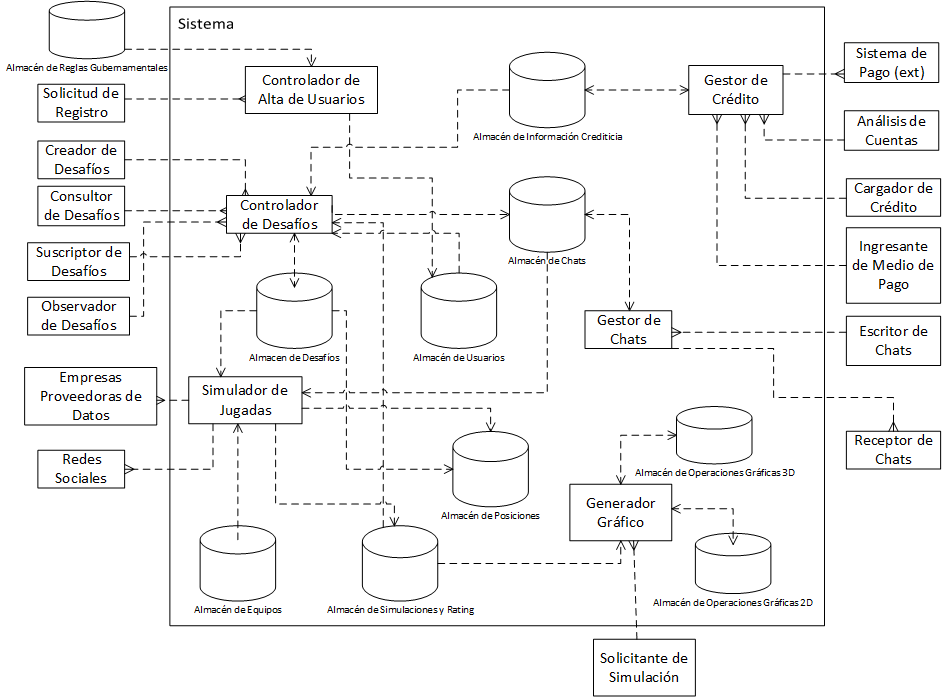
\includegraphics[scale=0.80,angle=90]{diagramas/arquitectura_general}
\label{fig:arquitectura_general}

En la figura \ref{fig:arquitectura_general} se ven los principales componentes del sistema, sobre los cuales se hace zoom en las secciones posteriores, además de los repositorios utilizados para nuestra solución.

\subsection{Controlador de Usuarios}
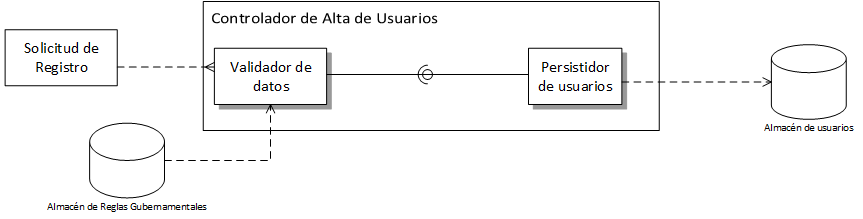
\includegraphics[scale=0.65]{diagramas/controlador_de_usuarios}
\label{fig:controlador_de_usuarios}

Toda \textbf{solicitud de registro} al sistema es recibida por el componente \emph{Controlador de Alta de Usuario}, que consta de tres etapas. 

El \emph{Validador de Datos} es la primera. Tal componente se encarga de validar las distintas posibilidades del usuario con respecto a las reglas gubernamentales establecidas en su país (que se consultan en el repositorio correspondiente). Es, básicamente, un filtro que le permite o no al usuario registrarse de acuerdo a la legislación vigente del territorio desde donde esté entrando al sistema.

Una vez validados los datos, si el usuario incluyó en su registro un método de pago, el \emph{Controlador de Alta de Medios de Pago} validará la información relativa al mismo con el servicio externo correspondiente, y la almacenará en el repositorio adecuado en caso de que sea correcta. El zoom de este componente se verá en la figura \ref{fig:gestor_de_credito}.

Por último, la tercer etapa, el \emph{Persistidor de Usuarios}, es el encargado, ya con todos los datos anteriores validados, de almacenarlos en el repositorio \emph{Almacén de Usuarios}, efectivizando así el registro del usuario.

\subsection{Controlador de Desafíos}
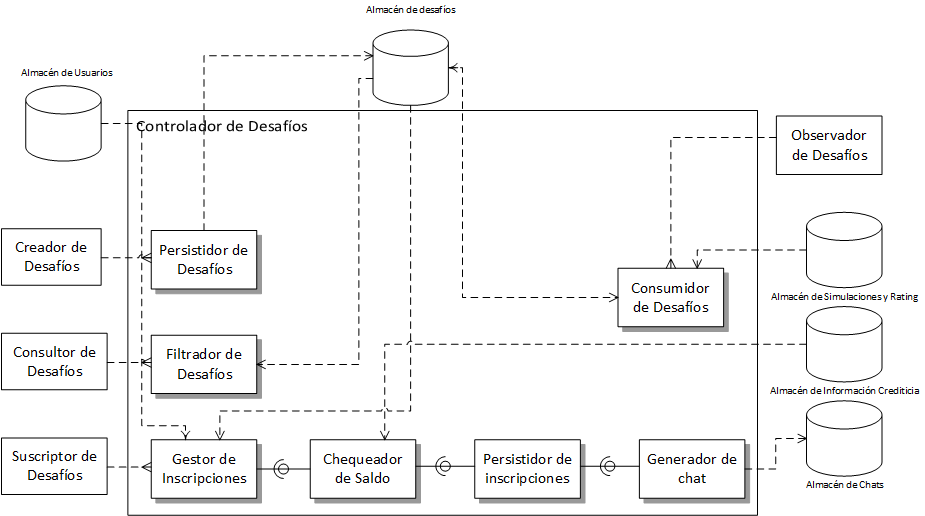
\includegraphics[scale=0.63]{diagramas/controlador_de_desafios}
\label{fig:controlador_de_desafios}

El \emph{Controlador de Desafíos} es ya un componente más complejo que el anterior, y ofrece diversas interacciones.

Por un lado, el \emph{Creador de Desafíos} se comunica con el \emph{Persistidor de Desafíos} y le comunica sus intenciones de crear un nuevo desafío; el \emph{Persistidor} almacena el nuevo desafío en el \emph{Almacén de Desafíos}, desde donde puede ser consultado por otros de los componentes.

Cuando un usuario desea consultar los desafíos a los que puede inscribirse (\emph{Consultor de Desafíos}), el \emph{Filtro de Desafíos} se encarga de interactuar con los datos del usuario y el \emph{Almacén de Desafíos}, para presentar la información solicitada de manera correcta.

Cuando un usuario desea inscribirse en un desafío (\emph{Suscriptor de Desafíos}), el \emph{Gestor de Inscripciones} es quien recibe la petición con todos los datos del usuario y el desafío en cuestión, y analiza si es posible o no cumplir con el pedido. Si lo es, se le transmite la información al \emph{Chequeador de Saldo}, quien validará -en caso de ser necesario- que el usuario cuente con el saldo suficiente para participar del desafío. 
Estos datos, luego, pasan por un pipe al componente siguiente, quien es el encargado de persistir la información del registro del usuario en el desafío elegido, dejando constancia de la inscripción.
Finalmente, el \emph{Generador de Chat} es quien inscribe al nuevo usuario en el chat global del desafío.

Por otro lado, las noticias y comunicaciones relativas a los desafíos, estén dirigidas a usuarios inscriptos o no, son leídas por el \emph{Consumidor de Desafíos}, quien es el encargado de, a partir de los datos de los desafíos generados y las simulaciones, ofrecer la información correspondiente a quien sigue un desafío (\emph{Seguidor de Desafíos}).